\documentclass[a4paper]{article}
\newcounter{QuestionNumber}
\setcounter{QuestionNumber}{1}

\newcommand{\Q}{
\textbf{Question \theQuestionNumber)}
\stepcounter{QuestionNumber}
}
\usepackage{amsmath,amssymb}
\usepackage{graphicx}
\usepackage{enumitem}
\usepackage[margin=1in]{geometry}
\usepackage{lipsum}
 \renewcommand{\familydefault}{\rmdefault}
\setlength{\parindent}{0pt}
\setlength{\parskip}{1em}
\begin{document}
\Large
\begin{center}
In the name of beauty

The 9th problem set solution of Optical Networks course

\hrulefill
\end{center}
%\section*{HW9: Dynamic Optical Networks}

%\textbf{General Hints and Descriptions}

%\textit{The main textbook for solving the following questions is Simmons' ``Optical Networks Design and Planning, Chapter 8''.}
%
%In the exercises below regarding transmission start-time calculations, consider only
%fiber propagation delays and switch configuration times (i.e., ignore processing
%delays). Take the speed of light in fiber to be $2 \times 10^8$ m/s. When a path is being set
%up, switches need to be configured at all intermediate nodes, as well as at the source
%and destination. If verification of path setup is not required, then the transmission
%start time at the source node is determined by the requirement that each switch in
%the path be configured by the time the initial transmission reaches it.
%When an exercise specifies that verification of path setup is required, assume that
%the verification message is initiated at the destination node upon completion of its
%own switch configuration. The verification message is sent to the source node; the
%intermediate nodes in the path do not forward the message until their own switch
%is configured.
%\begin{enumerate}
%\item

\Q

\begin{enumerate}[label=\alph*-]
\item
The propagation delay along each link is equal to
$$t_\text{prop}=\frac{1000km}{2\times 10^8}=5\text{msec}.$$
Path set-up has the following procedure. First, node A asks the PCE to calculate shortest path from itself to node H (the only PCE in the network). Node H immediately calculates the path and returns back the response to node A, totally in 30msec. Node A, having received the information, broadcasts the ``switch configuration'' message to all the nodes B,C,D and E. When in piplined mode, each node, receiving the ``switch configuration'' message, immediately forwards it to the other node, before starting its switch configuration. In an un-pipelined mode, each node must finish configuring its switch before forwarding the ``switch configuration'' message. Since all the mentioned nodes require an equal time for full switch configuration, node E is the bottleneck to the total elapsed time before the transmission from A to H is initiated. The ``switch configuration'' message takes 20msec to get to node H, 10msec is reserved for switch configuration, leading to a total of 30msec duration for the switch configuration of all other nodes on the path. With no path verification mechanism is employed, the total time of connection initiation is 60msec.

(With no pipelining, the elapsed time is increased for another 30msec, leading to 90msec in total.)
%If the PCE can only communicate with the source node, how long does it take from the receipt of the
%demand request to the time the source can begin transmission? Assume that the
%setup message from the source to the other nodes in the path is pipelined.
\item
With PCE advertising the response to every node directly, there is a 15msec delay before the response gets to nodes A and E (as the furthest two from the PCE) and a 10msec for switch configuration, leading to a total of $15+15+10=40msec$ delay.

%Repeat part (a), except assume that the PCE is allowed to directly communicate a
%setup message to each of the nodes in the path.
\item
Part(a): If node C is way lazier than the other nodes (!), there is a chance that it becomes the botteleneck. Let's see if this happens. There is a total of $10+40=50msec$ before node C switch is configured, whereas the same time for node E is 30msec. This difference in node C increases the total delay to 80msec.

Part(b): With a similar reasoning, node C is the bottleneck of switch configuration (you can simply check it for yourself!). The total elapsed time is 
$$
\underbrace{15}_{\text{A asks PCE}}
+
\underbrace{5}_{\text{PCE response gets to C}}
+
\underbrace{40}_{\text{C configures its switch}}=60msec.
$$
\end{enumerate}
%\begin{figure}[h!]
%\centering
%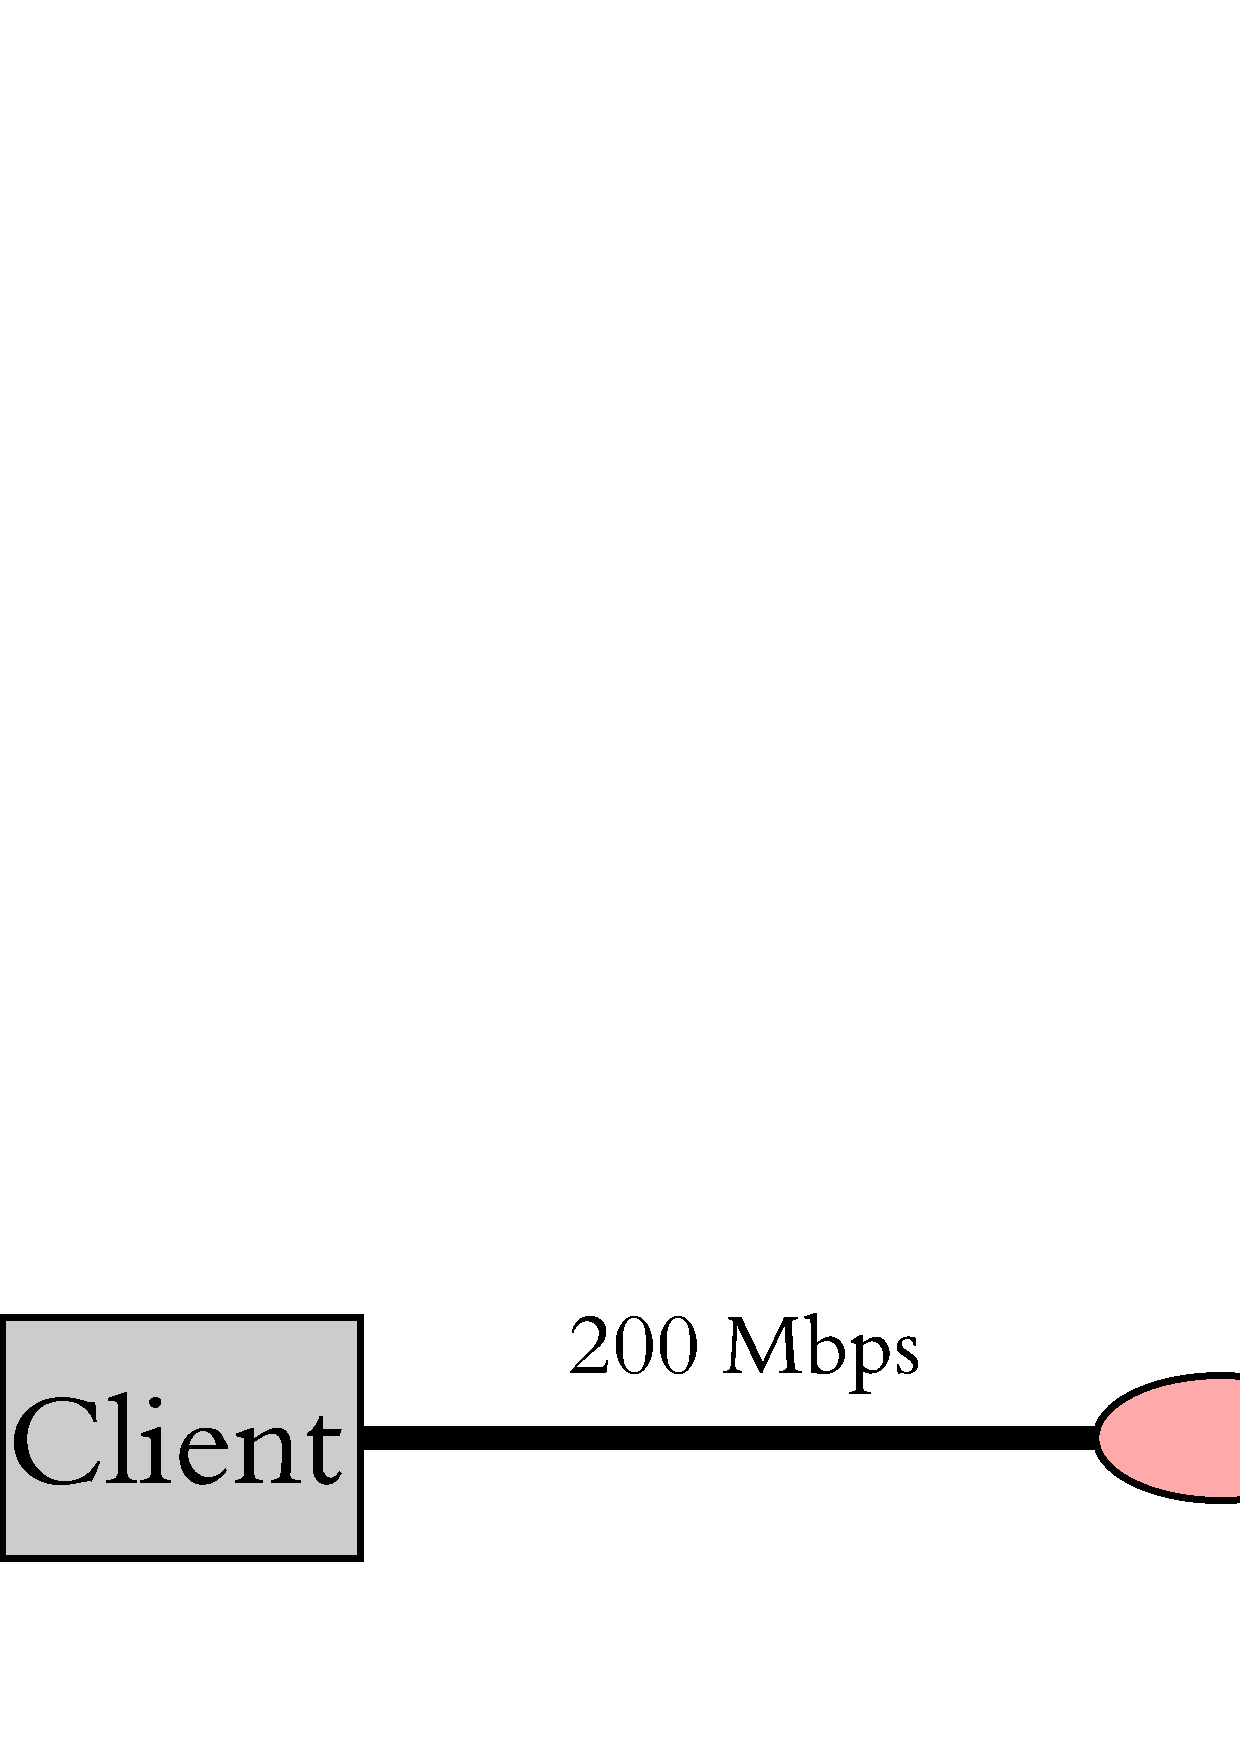
\includegraphics{Q1.PNG}
%\end{figure}

\Q

The procedure of question 1 is followed exactly, except considering the creation and transmission of verification message from each node of the path to node A. Node E is again a bottleneck (as is the furthest from node A).

\begin{enumerate}[label=\alph*-]
\item
The elapsed time is $60+20=80msec$.
\item
The elapsed time is $40+20=60msec$.
\end{enumerate}
%\item
%Repeat Exercise 1, parts (a) and (b), except assume that a verification message
%must be received by the source node indicating that the path has been
%properly configured.
%\item

\Q

The propagation delay along each link is increased to
$$
5msec\times 1.2=6msec.
$$
\begin{enumerate}[label=\alph*-]
\item
It takes 18msec for any packet arrival from node A to node H and vice versa. Hence, the total elapsed time is
$$
18+18+20+10=66msec.
$$
\item
The total delay is
$$
18+18+10=46msec.
$$
\end{enumerate}
%Repeat Exercise 1, parts (a) and (b), except assume that the grid topology
%shown in the figure holds only for the data plane. Assume that the control plane
%has a different topology such that the propagation delay between any two nodes
%or between a node and the PCE is 20 \% longer than in the data plane.
%\item 

\Q

%Consider a GMPLS-based implementation for establishing the AE demand
%shown in Exercise 1. Consider two scenarios, one where pipelining of the
%Resv message is not permitted, and one where it is permitted. Assume that a
%path setup verification message is not required before transmission can begin.
\begin{enumerate}[label=\alph*-]
\item
%If the switches at each node can be configured in 10 ms, how much sooner
%can the source begin transmission when pipelining is used?
In a GMPLS-based implementation, no (brainy!) node exists in the network and the path comutation resposibility is delegated to nodes in a distributed manner. It is reasonable to imply that node A saves for 30msec, since it does not require communication with node H. Therefore, A calculates the path independently. When pipelining is allowed, the total delay is
$$
20+10=30msec,
$$
while without pipelining, the delay is increased to
$$
5+10+5+10+5+10+5+10=60msec.
$$
\item
With the same method, pipelining requires
$$
10+40=50msec \quad,\quad \text{Since C is the bottleneck}
$$
whereas, without pipelining, we get to
$$
5+10+5+40+5+10+5+10=90msec.
$$

%If Node C
%requires 40 ms to configure its switch, instead of 10 ms, how much sooner can
%the source begin transmission when pipelining is used?
\end{enumerate}
%\item

\Q

%In the figure below, all vacant wavelengths in the links are denoted above them respectively. 
%\begin{figure}[tbh!]
%\centering
%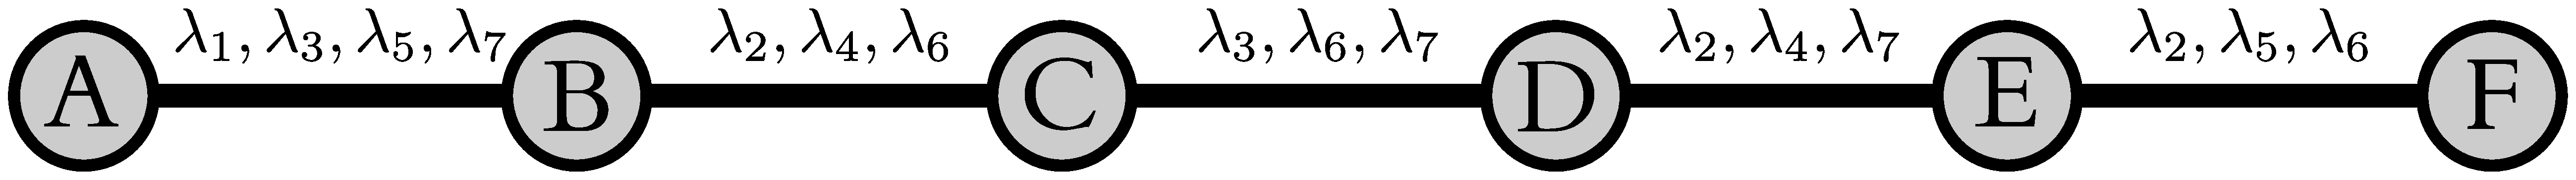
\includegraphics[scale=0.15]{lambda_bus.eps}
%\label{fig:Q5}
%\end{figure}
%
%When node A wishes to initiate a connection to node F through nodes B to D, it advertises a path message to node B by considering the available wavelengths on its outgoing link (link AB). Each intermediate node takes in the path message of its previous node and establishes a new path message containing available wavelengths in both the previous node path message and its available outgoing link. If no such free wavelength can be found, the node drops whatever information and alerts that a regeneration must take place. Then it chooses as path mesage, the free wavelengths on its outgoing link, regardless of the path message of its previous node. Finally reaching to destination, a Resv message is delivered back in the opposite direction and initiated at destination node. The Resv message contains the chosen wavelength on links for establishing connections.

%Answer the folowing questions:
\begin{enumerate}[label=\alph*-]
\item
\[
\begin{split}
&\text{Path Message}
\\&
A-B: \{\lambda_1,\lambda_3,\lambda_5,\lambda_7\}
\\&
B-C: \{\lambda_1,\lambda_3,\lambda_5,\lambda_7\}\cap 
\{\lambda_2,\lambda_4,\lambda_6\}=\{\}
\\&\text{Regeneration required at node B}
\\&B-C: \{\lambda_2,\lambda_4,\lambda_6\}
\\&C-D: \{\lambda_2,\lambda_4,\lambda_6\}\cap \{\lambda_2,\lambda_4,\lambda_6\}
=\{\lambda_6\}
\\&D-E: \{\lambda_6\}\cap
\{\lambda_2,\lambda_4,\lambda_7\}
=
\{\}
\\&\text{Regeneration required at node D}
\\&D-E: \{\lambda_2,\lambda_4,\lambda_7\}
\\&E-F: \{\lambda_6\}\cap
\{\lambda_2,\lambda_4,\lambda_7\}
\cap\{\lambda_2,\lambda_5,\lambda_6\}
=\{\lambda_2\}
\end{split}
\]

Once the path message is initiated on all links, a resv message confirms the allowed, free wavelengths on all links.
\[
\begin{split}
&\text{Resv Message}
\\&F-E: \{\lambda_2\}
\\&E-D: \{\lambda_2\}
\\&D-C: \{\lambda_6\}
\\&C-B: \{\lambda_6\}
\\&B-A: \text{either one of $\{\lambda_1\}$, $\{\lambda_3\}$, $\{\lambda_5\}$ and $\{\lambda_7\}$}
\end{split}
\]

\item 
The failure returns to node A once either there are no free wavelengths on link EF or there is no regeneration equipment available on node E.
\end{enumerate}
%\item




%\end{enumerate}
\end{document}


